\documentclass[prl,aps,twocolumn,showpacs,twocolumngrid,superbib]{revtex4}


\usepackage{graphicx}
\usepackage{amsfonts}
\usepackage{amsmath}
\usepackage{bm}
\usepackage{alltt}
\usepackage{fancyhdr}
\newcommand{\bms}[1]{{\boldsymbol #1}}
\renewcommand{\thefootnote}{\fnsymbol{footnote}}

%\draft
%\tighten
\pagestyle{fancy}

\begin{document}

\title{
A New View on the Geometry Optimization of Large Molecules\footnotemark[1]}

\author{K\'aroly N\'emeth\footnotemark[2]}
\author{Matt Challacombe}

\affiliation{Theoretical Division, Los Alamos National Laboratory, Los Alamos, NM 87545, USA}

\date{\today}

\begin{abstract}
{
This article peresents a new, efficient alternative to well established
geometry optimization algorithms. The new alternative is based on
fitting gradient surfaces in terms of curvilinear 
internal coordinates and 
determining the roots of the fitted surface. Due to the efficient 
vibrational decoupling of the curvilinear coordinates the 3N-dimesional
optimization problem splits into a quasi non-interacting
set of approximately 3N one-dimensional optimization problems, 
similarly to the self-consistent mean-field concepts of physics.
This allows for robust, linear scaling implementation of geometry optimizers.
}

\smallskip
\noindent{\bf Keywords}: 
geometry optimization, linear scaling, 
curvilinear internal coordinates, fitting
\end{abstract}
 

\maketitle

\footnotetext[1]{LA-UR-04-1097}
\footnotetext[2]{\tt KNemeth@LANL.Gov}

\section{Introduction}
The optimization of molecular structures is one of the most frequent
tasks carried out by computational chemists. 
Structures of large molecules have been optimized so far
only with the use of empirical force-fields, or at most with 
semi-empirical electronic structure theories 
\cite{Stewart_crambin_opt,Schlegel_plasminogen_opt}. However, many important phenomena
can be understood only poorly on these low levels of the theory. 
Such phenomena are e.g. the structural changes of large molecules, 
when beeing put from one solvent into another, the mechanisms of 
enzymatic reactions, the selectivities of ion-channels, etc. 
Geometry optimization is one of the simplest tools to start studying 
these phenomena, since it needs only energy gradients, as input, but 
leads to a welth of relevant structural information.
Not only equilibrium structures, but also transition states and reaction
paths can be determined with the help of efficient optimizers 
\cite{nudged_elastic_band}.

With the advent of linear scaling electronic structure techniques 
\cite{Goedecker99}
energies and gradients are available for large molecules on demanding
levels of the theory. However, even linear scaling can have 
a considerable computational cost on large molecules. In order to
make the computational cost smaller, efficient optimizers are
needed, which are suitable for large molecules.

The present paper reveals a new concept for the optimization of
molecular geometries, which is especially suitable for the
optimization of large molecules and performs equally well in the
domain of small molecules, too. It can be easily implemented
in a linear scaling fashion, too.
The new concept is based on the availability of internal coordinate
gradients for large molecules - a result of recent developments
\cite{paizs_coordtrf1,nemeth_coordtrf1,paizs_coordtrf2,nemeth_coordtrf2,billeter_coordtrf,andzelm_coordtrf,kudin_coordtrf}.
Our observation is that internal coordinate gradients show clear
tendencies during the optimization process and these tendencies can be revealed
by curve fitting in one-dimension, over internal coordinate value and gradient
data pairs. For an illustration of this concept,
see Fig. \ref{NH3outp6} for a typical progression of internal coordinate
gradients. The roots of the fitted curve reveal the expected location
of the minimum. This concept can be realized only in terms of
internal coordinates which are representations of chemical entities, such as
bond lengths, bond angles and torsional angles. Cartesian
coordinates do not provide the same clear progression.
\begin{figure}[h]
%\resizebox*{3.5in}{!}{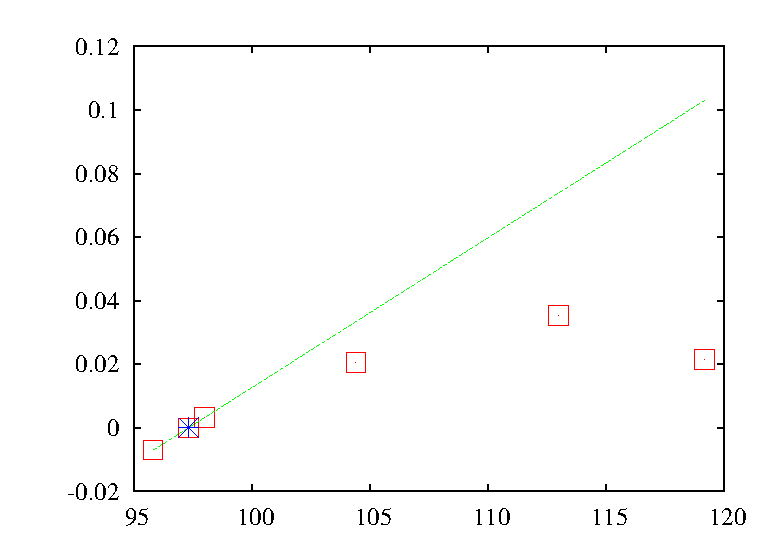
\includegraphics{1_6_6_Data.eps}}
%\resizebox*{3.5in}{!}{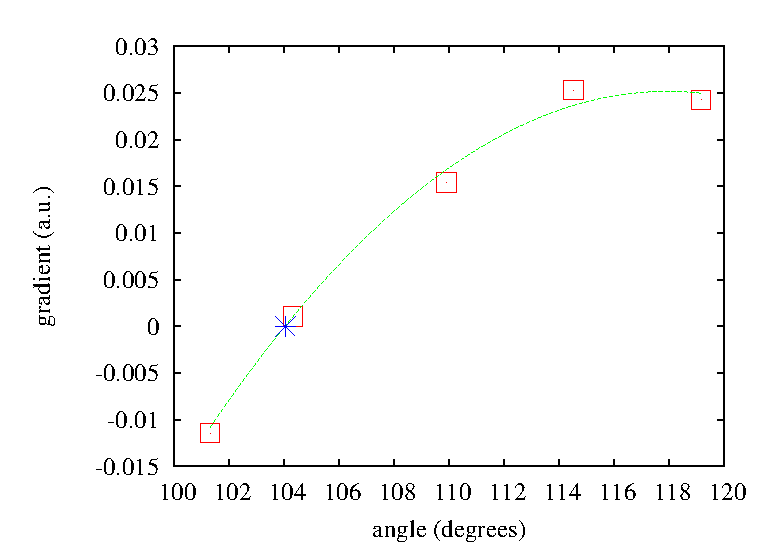
\includegraphics{1_5_6_Data.eps}}
\resizebox*{3.5in}{!}{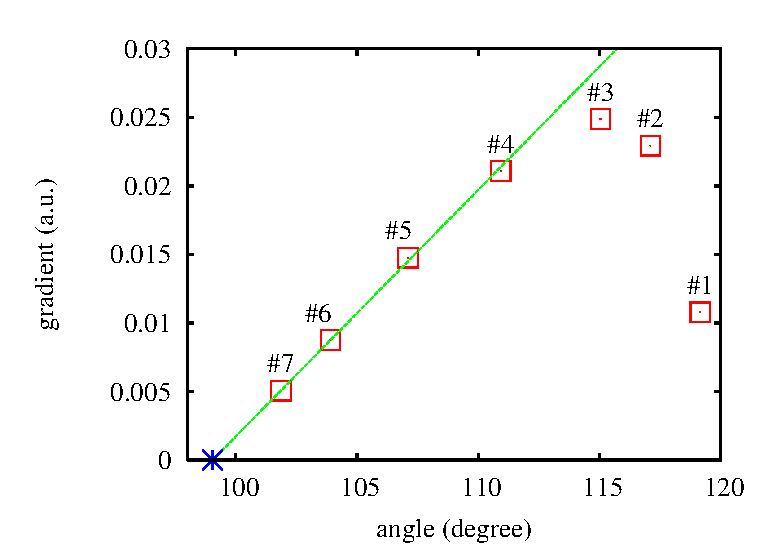
\includegraphics{1_7_6_Data.eps}}
\caption{
\small  
Progression of gradients on a valence angle bending coordinate of
ammonia. The optimization was started from near planar geometry, i.e.
from the vicinity of a transition state, and converged to a local 
minimum of the potential energy surface. The numbers in the picture
indicate the sequence of optimization steps. The dotted line represents
a quadratic fit, the star the predicted location of the minimum.
\label{NH3outp6}
}
\end{figure}

\section{Traditional techniques}
In the last three decades the so-called internal coordinate 
optimizers became standard tools of geometry optimization when energies 
and forces are calculated by electronic structure theory 
\cite{Pulay_natural_internals}.
Internal coordinates describe the internal motions of molecules 
by displacements of chemical entities, such as bond-stretches, 
valence angle bendings and torsions of dihedral angles. These 
coordinates are curvilinear, since they can be composed
as non-linear functions of the Cartesian coordinates of atomic nuclei.

An important property of these chemical internal coordinates
is that they significantly reduce the harmonic and higher order 
vibrational coupling, as compared to Cartesian ones 
\cite{pulay_dynamics,Baker_deloc_1}. 
Even if accurate harmonic force-constants are available, 
internal coordinates are superior for geometry optimization, 
since anharmonic effects are
usually large, especially far from the minimum 
\cite{Baker_deloc_1}. 

A rough estimate of internal coordinate force constants is usually 
enough for an efficient geometry optimization of small molecules
\cite{bakken,fogarasi_diaghess}, however it is not satisfactory
for larger molecules of complex structure.

In order to get more accurate curvature information about the 
potential energy surface the so-called Hessian-matrix update schemes
are used \cite{RFletcher}. 
Hessian matrix update schemes are derived from the assumption of a 
harmonic potential energy surface. 
The success of Hessian update schemes is based on, that for geometry 
optimization a reasonable estimate of the Hessian 
is enough to bring the molecule to a local optimum by 
quasi-Newton steps. 

The updated Hessian matrices require ${\cal{O}}(N^{2})$ storage, thus
their use becomes a computational bottleneck for large molecules.
There are a few approaches to overcome this limitation.
The most widely used one is the Limited Memory BFGS (LBFGS) 
technique of Nocedal
{\it et.al.} \cite{nocedal_lbgs}. This technique does never explicitely 
construct the full Hessian matrix. Instead, it carries out all 
the necessary operations by an implicite application of the Hessian
via its component vectors. LBFGS
has the limitation that it can use only a small number of remembered
steps.
Another efficient approach has been constructed very recently by Bofill,
Anglada et.al. \cite{bofill_lanczos}. This approach is similar
to LBFGS in the sense that it avoids the use of the explicite
Hessian, but it can calculate necessary eigenvectors of the 
Hessian by a Lanczos-type algorithm. A
similar approach is the ${\cal{O}}(N^{2})$ scaling iterative
scheme of Schlegel and Farkas \cite{schlegel_on2iter}.
In Stewart's approach, an update
formula of the inverse Hessian has been used, and the full explicite
Hessian has been truncated by spacial thresholding and stored in a 
sparse matrix fashion \cite{Stewart_crambin_opt}. 
The reported performance
of Stuart's scheme was rather poor on large molecules.

The efficient use of internal coordinates for large molecules has 
been limited by another important factor. That is the coordinate
transformation problem, which must be carried out very frequently
to transform Cartesian vectors and curvilinear internal ones into each
other. This problem has found a linear scaling solution   
only in recent developments 
\cite{paizs_coordtrf1,nemeth_coordtrf1,paizs_coordtrf2,nemeth_coordtrf2,billeter_coordtrf,andzelm_coordtrf,kudin_coordtrf}. 


\section{A new concept}
In the present article we introduce a new concept 
to molecular geometry optimization. We call this approach the
Optimization through Gradient Curve Fitting (OGCF) technique. 
This new approach is very simple
to implement, scales fully linearly with system size 
and is very efficient for both small and large molecules.

The new algorithm is based on the fact that
normal mode gradients are linear functions of the normal mode values 
on harmonic potential energy surfaces. 
In the process of geometry optimization the goal is to reveal the roots
of these lines, where all gradients become zero. In order to 
find these roots, first a few points should be determined from each
lines, then the roots can be revealed by line-fitting. 

In a realistic case neither the potential energy surface is 
harmonic, nor the normal modes are available. However, it is always
possible to construct internal coordinates based on the chemical
intuition, and these internal coordinates will have a reduced
vibrational coupling, similar to normal modes. 
In this sense the internal coordinates represent an a-priory
approximation to normal modes.
The corresponding
gradient curves will not be straight lines for internal coordinates,
but they still represent stronger or weaker tendencies, as the molecular
structure walks on the potential energy surface, e.g. during geometry
optimization. 
See Fig. \ref{NH3outp6} for a typical progression of internal
coordinate gradients during geometry optimization.
These tendencies can again be revealed by fitting curves to the
coordinate-gradient data pairs. For each internal coordinate 
the root of the fitted curve then 
serves as a new estimate for the coordinate value where the gradient
should become zero. Repeating this fitting process can finally
reveal a local optimum of the the potential energy surface.
The analogy with the case of the normal modes suggests a possibility
for quadratic convergence, as soon as the rate of vibrational
coupling is small enough.
It is also important to note, that the fitting process happens
with weighted data points. The weights reflect local tensions
of the molecule and are calculated in a simple way, as described below.
The fitting of gradient surfaces has already been applied to 
the parametrization of empirical
force-fields for the case of small molecules
\cite{force-field-fitting,force-matching}, however it 
has not been investigated for the purpose of geometry optimization yet.

\section{Implementation}
\subsection{Choice of internal coordinates}
The basis of recognizing internal coordinates is the recognition
of the bonding scheme. This is being done at each new geometry.
The bonding scheme is recognized in a linear scaling fashion, via
a divide-and-conquer algorithm. The topology of the bonding scheme
is stored in a sparse matrix. These sparse matrices are summed
up over the few most recent geometries, in order to provide
the topology of a merged bonding scheme.

Then, based on the topology matrix of the merged bonding schemes,
all other primitive internal coordinates, such as bond angles,
torsions, linear bendings and out-of-planes are recognized. Torsions
are selected so that each bond will be associated with a single
torsional coordinate.
The merger of bonding schemes is important, since we need to
generate internal coordinates suitable for the coordinate
transformations of each recently passed Cartesian geometry.

\subsection{Preparing the data points}
Cartesian coordinates and the corresponding Cartesian gradients
of the few, typically seven most recent geometries are read from 
disk. Based on the most recent definition of the bonding scheme
they are transformed into internal coordinate representation.
The coordinate transformation is carried out as described in Ref.
\cite{nemeth_coordtrf1}, while the necessary intermediate sparse
matrices of the coordinate transformation are regenerated. This
is a very inexpensive step, due to the extrem sparsity
of the matrices.
Thus the primary objects of the proposed geometry optimization
are created. For each remembered geometry the internal coordinates
and their gradients are now available.

In order to avoid problems due to the periodicity of torsional angles,
reference points are used, eg. the torsional angle values 
of the most recent geometry. Each torsional angle is
set to its periodic equivalent 
closest to the reference point, by a 
shift of $\pm 2\pi$, while its gradient value does not change.

\subsection{Curve fitting with weights}
At this point for each individual internal coordinate we have a set of 
coordinate - gradient pairs, such as the one presented in 
Fig. \ref{NH3outp6}. These data pairs indicate the progression
of the gradient during the few most recent optimization steps.
They are now used to fit a curve as mentioned above.

The curve-fitting happens through 
well established and robust algorithms, which are available in standard 
computational libraries \cite{slatec}. 
It is important to note
that data points are weighted before the fit. The weights, 
$w_{k}^{(i)}$, are
measures of the stuctural tension in the vicinity of the $k$-th internal
coordinate at the $i$-th geometry. They account for the effect of the 
environment on the $k$-th internal coordinate. 
The weights are computed as
\begin{equation}
w_{k}^{(i)} = \left[ \sum_{l} g_{l}^{(i)} \frac{1}{|H_{ll}^{}|} g_{l}^{(i)} \right]^{-1} ,
\end{equation}
where $l$ indicates the internal coordinates which have atoms in common
with the $k$-th internal coordinate, i.e. which are in the spacial 
vicinity of the $k$-th coordinate. 
$H_{ll}^{}$ is an estimate
of the diagonal matrix element of the Hessian for the $l$-th 
internal coordinate. $H_{ll}^{i}$ is calculated as the local tangent
of the gradient curve of a primary fit. 
This primary fit is done for each internal coordinates with 
the weights $w{'}_{k}^{(i)} = 1/g_{k}^{(i)2}$ usual to 
estimate relative errors.

The statistical F-test is used to decide about the order of the fit,
as implemented in the fitting program \cite{slatec}.
So far no higher than cubic fit has been considered. The roots
of the fitted curves can be found analytically. In practice,
almost exclusively linear fit was recommended by the F-test during
the test calculations.

The topology matrix, neded to determine which internal coordinates
are neighbouring each other, is given by 
the sparse $G_{i}=BB^{t}$ matrix that is easy to compute from the
sparse vibrational $B$ matrix. We have considered more delocalized 
interactions as well, such as the topology offered by $G_i^2$,
but they turned out not to provide any significant improvement in our
test calculations so far.


\subsection{Minimum or transition state?}
In case the gradient curve has a negative tangent at the position
of the root, it is an indication for a transition state. 
Eg. in Fig. \ref{NH3outp6} the tangent of the gradient curve 
is negative in the vicinity of the planar
structure (structure \#1). This should be so, since the planar
ammonia represents a transition state. The tangent of the gradient 
curve thus offers a
convenient tool to control convergence to minima or transition state.
We plan to elaborate a transition state finding tool based on this 
principle. In the present article we restrict the discussion
to the localization of minima. Whenever the local tangent  
of the gradient curve
is negative, the optimizer moves the actual geometry away from 
the transition state. This way those transition states 
can be avoided, which are localized well on a few internal coordinates. 
In the present paper we do not consider the case of more 
delocalized transition states which are in principle possible,
however rarely occure. Combined internal coordinates, such
as the natural internal ones \cite{Pulay_natural_internals} or the
delocalized internal ones \cite{Baker_deloc_1} hold the possibility
of revealing more delocalized transition states by the
curve fitting technique. The analysis of Wales {\it et.al.} 
\cite{Wales_saddlepoint}
gives a numerical insight into the problems of controlling
convergence to a minimum without an accurate Hessian.

\subsection{Initial steps}
In the first two steps of the optimization
process a scaled internal coordinate steepest descent step is used
with the usual diagonal Hessian estimates of
0.5 a.u. for stretchings, 0.2 a.u. for bendings and 0.1 a.u.
for torsions. The use of the OGCF optimizer could start in the
second geometry, however the cruder diagonal Hessian steps have less
step size limitation in the second step, resulting in a slightly
better overall performance for some of our test sets.

\subsection{Step size control}
In case the optimizer makes an extrapolation step towards the predicted
minimum, the length of this step is limited by the range of the
data points used for the fit. Step sizes are limited to be smaller
than 0.3 a.u., similar to what is used by other optimizers 
\cite{eckert}.
For larger molecules of more complex structure 
it is advantageous to restrict
the stepsize to be 0.15 a.u., instead of the usual 0.30 a.u. 
in order to proceed more carefully.

\subsection{Iterative back-transformation}
Once the predictions are made, the required new values of the internal
coordinates are passed in to the iterative back-transformation
(see e.g. Ref. \cite{nemeth_coordtrf1})
to generate the new set of Cartesian coordinates. Note, that no
redundancy projector is used in our approach to pre-process the
required internal coordinate displacements. In case the iterative 
back-transformation would fail, it will repeat the process with 
half of the original
internal coordinate displacements required. If the repeated action 
would also fail that indicates an incomplete set of internal coordinates
and the programm stoppes. For large molecules this can often be the case
if hydrogen-bonds or Van-der-Waals contacts have not properly been 
accounted for. However, it is easy to avoid this case by properly 
setting up the internal coordinate recognitions.

\section{Performance}
The performance of this initial implementation of the OGCF optimizer
has been tested on a 
series of small molecules, called Baker's test set \cite{bakerstest}.
At convergence, the maximum remaining Cartesian
force vector had a length less than $3\times10^{-4}$ a.u. for each
atom. This criterion is somewhat tighter then the original requirements
of Ref. \cite{bakerstest}, stating the same for the Cartesian X,Y and Z
components of the force. The energies of the optimized
structures have been reproduced to all digits given in 
Ref. \cite{bakerstest}.

Table \ref{Bakers_test} lists all the test results
in order to convince
the reader, that our new concept of geometry optimization
works as well on small molecules as the best implementations
of traditional algorithms.
Note, that the alternative coices of the
internal coordinate systems can easily change the number
of optimization steps by at least $\pm$10\%.
We expect further improvement by the application of combined    
internal coordinates, such as the natural internal ones or the 
delocalized ones. 
Note, that our results have been achieved without any use
of traditional convergence acceleration algorithms, such as 
geometric DIIS \cite{Pulay_GDIIS}, which are standard tools of
traditional optimizers \cite{Farkas_GDIIS}.

\begin{table}[h]
%\squeezetable
\caption{
Geometry optimization steps of small molecules (upto 30 atoms)
of the Baker's test set. Calculations have been carried out 
with the Hartree-Fock model in STO-3G basis set.
All calculations used standard primitive internal coordinates,
except the one by Bakken {\it et.al.}, which used extra redundant
ones.
}
\label{Bakers_test}
\begin{tabular}{lccccc}
\toprule
Molecule               & Present  & Bakken & Eckert  & Lindh &  Baker  \\
         & work & {\it{et al.}} & {\it{et al.}} & {\it{et al.}} &    \\
         &(OGCF) &  \cite{bakken} &  \cite{eckert} & \cite{lindh} &  \cite{bakerstest} \\
\colrule
Water                  &   4    &   4    &    4    &    4   &   6     \\
Ammonia                &   4    &   5    &    6    &    5   &   6     \\
Ethane                 &   4    &   3    &    4    &    4   &   5     \\
Acetylene              &   4    &   4    &    6    &    5   &   6     \\
Allene                 &   3    &   4    &    4    &    5   &   5     \\
Hydroxysulphane        &   7    &   7    &    7    &    8   &   8     \\
Benzene                &   2    &   3    &    3    &    3   &   4     \\
Methylamine            &   4    &   4    &    5    &    5   &   6     \\
Ethanol                &   5    &   4    &    5    &    5   &   6     \\
Acetone                &   5    &   4    &    5    &    5   &   6     \\
Disilyl ether          &   9    &   8    &    9    &   11   &   8     \\
1,3,5-trisilacycl.     &   6    &   9    &    6    &    8   &   8     \\
Benzaldehyde           &   4    &   4    &    5    &    5   &   6     \\
1,3-difluorobenz.      &   4    &   4    &    5    &    5   &   5     \\
1,3,5-trifluorob.      &   3    &   4    &    4    &    4   &   5     \\
Neopentane             &   5    &   4    &    4    &    5   &   5     \\
Furan                  &   6    &   5    &    6    &    7   &   8     \\
Naphtalene             &   6    &   5    &    6    &    6   &   5     \\
1,5-difluoronapht.     &   6    &   5    &    6    &    6   &   6     \\
2-hydroxibicyclop.     &   8    &   9    &    9    &   10   &  15     \\
ACHTAR10               &   9    &   8    &    9    &    8   &  12     \\
ACANIL01               &  11    &   7    &    8    &    8   &   8     \\
Benzidine              &   8    &   9    &    7    &   10   &   9     \\
Pterin                 &  14    &   8    &    9    &    9   &  10     \\
Difuropirazine         &   7    &   6    &    7    &    7   &   9     \\
Mesityl oxide          &   5    &   5    &    6    &    6   &   7     \\
Histidine              &  10    &  16    &   14    &   20   &  19     \\
Dimethylpenthane       &   7    &   9    &   10    &   10   &  12     \\
Caffeine               &   7    &   6    &    7    &    7   &  12     \\
Menthone               &  16    &  12    &   10    &   14   &  13     \\
\colrule
Total                  & 193    & 185    &  196    &  215   & 240     \\
\botrule
\end{tabular}
\end{table}

While retaining the same efficiency for small molecules, our technique
is fully linear scaling as opposed to any other internal 
coordinate optimizers reported so far. In addition, it is far simpler
to implement then any traditional alternatives.
This allowes the fast and efficient 
extension of geometry optimization 
to large molecules, where scaling issues are important.
In order to illustrate the performance of our optimizer on large
molecules, we show the convergence of the molecular total energy
during the course of the optimization of a 257 atom
fragment of Protein Kinase A, in Figs. \ref{logn-logde} 
and \ref{order-of-conv}. Ten periferial atoms have been 
constrained, in order to mimic the rest of the enzyme, 
all other atoms have been allowed to move.
The optimizations have been carried out 
using MondoSCF \cite{MondoSCF}, a linear scaling electronic structure
program system, the PBE density functional model and 
STO-2G basis set, with 0.1 milliHartree resolution of the energies.
The convergence was smooth with minor jumps in the energy.

Iterative processes are characterized by the order, $n$
and the rate, $c$ of the convergence. For the convergence of the
energy this reads:
\begin{equation}
\frac{|E_{i+1}-E_{opt}|}{|E_{i}-E_{opt}|^n}=c ,
\end{equation}
with $E_{opt}$ being the optimum energy and $E_{i}$ the energy
at the $i$-th geometry.
A first order convergence is typical for the bulk of the optimization
of larger molecules. For smaller molecules, like the ones of Baker's
test set, the order of convergence is between linear and quadratic,
with an acceleration towards convergence. Note, that in the case
of first order convergence the rate of the convergence is still
smaller than one, which results in decreasing error.
\begin{figure}[h]
\resizebox*{3.5in}{!}{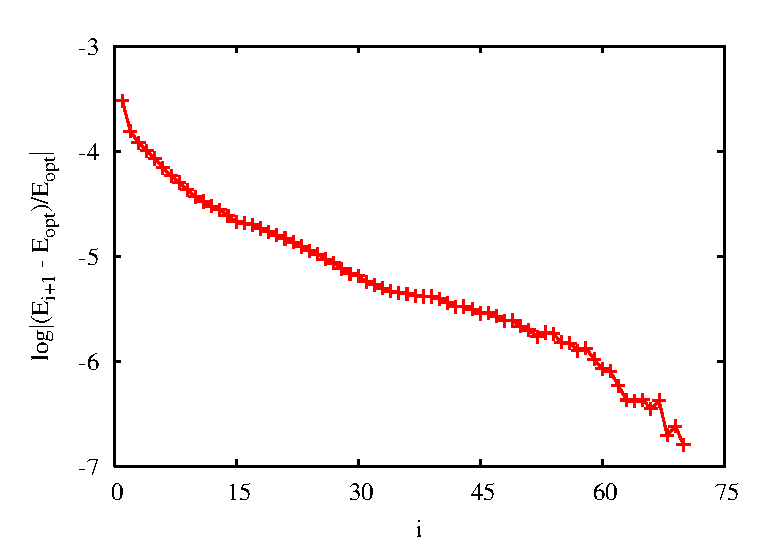
\includegraphics{curve3.eps}}
\caption{
\small  
The error of the energy has an exponential decline during
the optimization of a 257 atom protein kinase A fragment. 
$i$ denotes the serial number of steps,
$E_{opt}$ is the optimum energy.
\label{logn-logde}
}
\end{figure}
%
%
%
%
\begin{figure}[h]
\resizebox*{3.5in}{!}{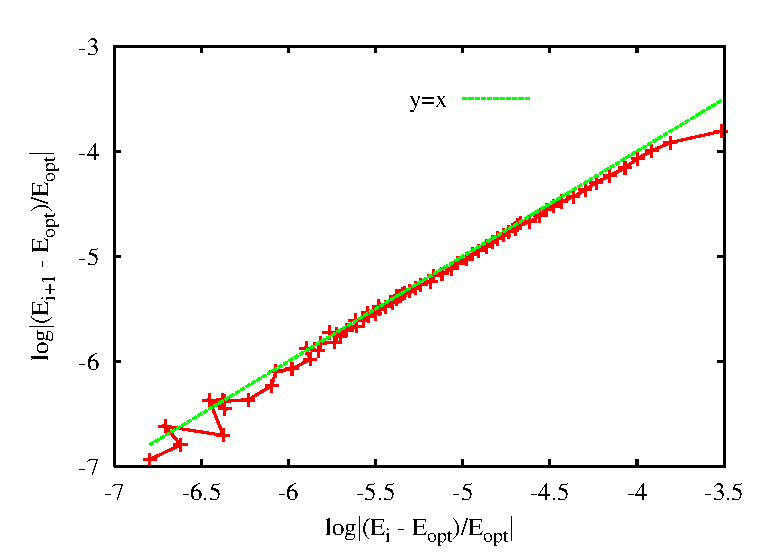
\includegraphics{curve2.eps}}
\caption{
\small  
Relative errors of the energy show linear improvement.
Thus, the convergence is of first order. Higher order
convergence can be expected only beyond the milliHartree
energy resolution for this molecular size.
\label{order-of-conv}
}
\end{figure}

\section{Summary}
In this article we have presented a new concept
to the optimization of molecular structures.
We have shown, that internal coordinates representing chemical 
entities can efficiently be optimized, without
ever accounting for explicite vibrational couplings, as traditional
optimization techniques do. This allowes an efficient
extension of quantum-level modeling to geometrical processes
of biomolecules, such as enzymatic reactions, macroscopic quantum 
effects in ion-channels or solvent effects on biomolecules.
Our technique can also be used
to provide simple and accurate updates of force-fields
for molecular dynamics simulations, based on the availability of
quantum-mechanical forces.

\begin{acknowledgments}
K. N{\'e}meth gratefully acknowledges to 
{\"{O}}. Farkas (Budapest) for 
providing the Cartesian coordinates of the Baker's test set and to
B.P. Uberuaga (Los Alamos) for calling our attention to Ref. 
\cite{force-matching}.
\end{acknowledgments}

\bibliography{mondo_new}
\end{document}
